\chapter{Industry Guidance on Collaboration Processes} % Main chapter title

\label{Chapter8} % Change X to a consecutive number; for referencing this chapter elsewhere, use \ref{ChapterX}

\lhead{Chapter 8. \emph{Industry Guidance}} % Change X to a consecutive number; this is for the header on each page - perhaps a shortened title

%----------------------------------------------------------------------------------------
%	CHAPTER INTRO
%----------------------------------------------------------------------------------------

This chapter summarises some of the guidance that is provided by the industry and government for the collaboration of building services engineers.

%----------------------------------------------------------------------------------------
%	SECTION 1
%----------------------------------------------------------------------------------------

\section{Authoritative Documents}

There is a myriad of documents published by the AEC industry and the government that provide guidance on how construction professionals should communicate and collaborate with each other.
This especially since a call for collaboration was made in the Latham and Egan Reports, and the Cabinet Office mandated BIM Level 2 on public sector projects in 2011.
Some of the main guides that concern building services engineers and that have been analysed for the purposes of this thesis are displayed in red on the timeline in Figure \ref{timeline}.
%The documents that dictate the processes of work (i.e. activities and deliverables for every work stage) or building services engineers are displayed in \hl{red} in the timeline in figure \ref{timeline}.
Most of the guides are aligned with the RIBA PoW 2013, except for PAS 1192-2 which aligns itself with the CIC Scope of Services stages.
However, the CIC Scope of Services stages are more or less aligned with RIBA PoW 2013, as shown in Figure \ref{fig_pow_alignments}.
The purpose and content of the main guides are outlined below:
\begin{itemize}
    \item \textbf{PAS 1192-2:2013} \citep{PAS1192}: A standard that provides guidance for information requirements, generation and flow using BIM during the capital expenditure (CAPEX) phase of construction projects.
    \item \textbf{BG 6} \citep{BG62014}: 
    %Provides an \say{aide-memoire of design activities, first where this clarifies the duties listed in standard forms of agreement for appointing design consultants, and second where allocation of design activity is either currently overlooked or is open to debate.} // 
    %This is the building services engineer’s `bible' that provides guidance on their activities, and drawing and model definitions for each stage of the design and construction process. // 
    A technical guide that provides a framework for allocating many of the design activities, in connection with the building services aspects of a construction project, to the different members of a project team. It provides standard pro-formas, as well as exemplary drawings and models for each stage of a project.
    \item \textbf{CIBSE Digital Engineering (DE) Series} [\citeauthor{DE2}, 2016-17]: A series of documents that provide practical guidance for the full built environment supply chain (not just building services engineers) on how to deliver a project using BIM.
    \item \textbf{ACE Schedule of Services; MEP} \citep{ACE2017}: A document that sets out the services to be performed by MEP engineers on projects.
\end{itemize}


\begin{figure}[htbp]
	\centering
	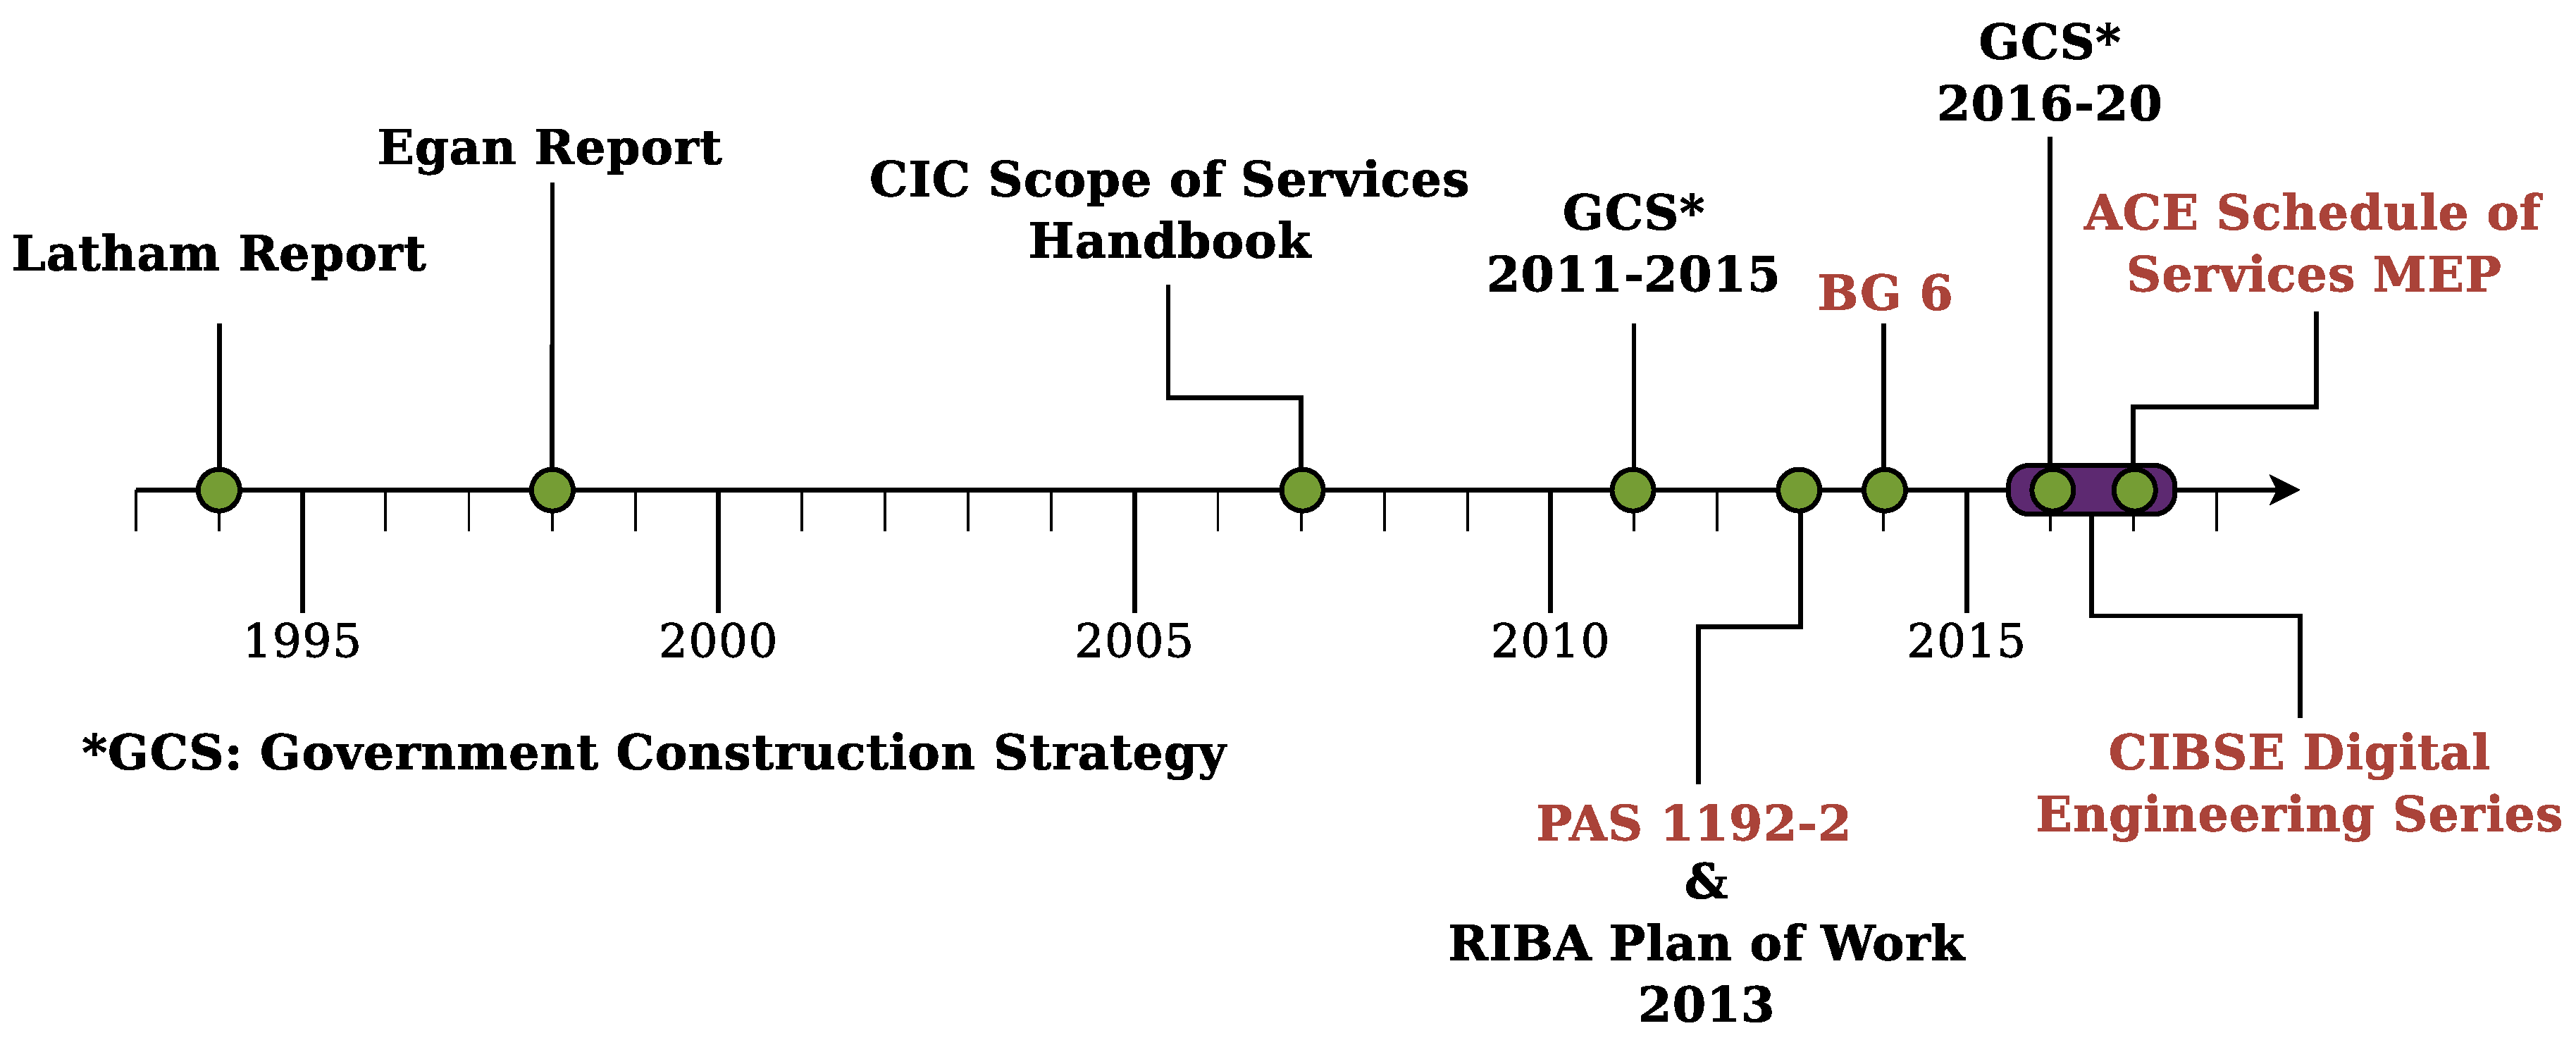
\includegraphics[width=\textwidth]{figures/Timeline2.eps}
	\rule{\textwidth}{0.5pt} % use line???
	\caption[Timeline of government construction strategies, and industry reports and guides since 1994.]{Timeline of government construction strategies, and industry reports and guides since 1994. The main guides that concern building services engineers are displayed in red.}
	\label{timeline}
\end{figure}


\begin{figure}[htbp]
	\centering
	\includegraphics[width=\textwidth]{figures/PoW_Alignments.png}
	\rule{\textwidth}{0.5pt} % use line???
	\caption[Alignment of RIBA PoW 2013 and CIC Scope of Services stages]{Alignment of RIBA PoW 2013 and CIC Scope of Services stages \citep{CIC2007, ArchitectsJournal}.}
	\label{fig_pow_alignments}
\end{figure}


The following two sections summarise the main findings regarding the collaboration of building services engineers regarding consultant-to-contractor handovers and levels of definition.



\begin{comment}
\textbf{What did I find out?}
The documents, although a bit messy and not speaking exactly the same language or using exactly the same PoW, were more in agreement than I expected.
They all admit to the flexibility required for building services engineers during Stage 4. In fact, they state that contractors can intervene at even earlier stages of the process. 
Despite this (when the consultants/ contractors are in charge), the activities/ deliverables/ services remain the same.
\end{comment}


%----------------------------------------------------------------------------------------
%	SECTION 2
%----------------------------------------------------------------------------------------

\section{Consultant-to-Contractor Handover Points}

The AEC industry seems to agree on the necessity for flexibility
regarding the handover points between building services consultants and contractors \citep{BG62014, ACE2017, CIC2007, RIBAPlan}.
The handover points vary according to the selected procurement routes, as exemplified in Figure \ref{fig_BG6_handover_pts}.
The BG 6 \citep{BG62014}, ACE Schedule of Services \citep{ACE2017} and RIBA PoW 2013 \citep{RIBAPlan} stress on the importance of understanding the selected procurement route and clarifying the allocation of responsibilities between the consultant and contractor at an early stage.
According to \cite{RIBAPlan}, ``The Design Responsibility Matrix \footnote{A Design Responsibility Matrix is a \say{matrix that sets out who is responsible for designing each aspect of the project and when. [\ldots] The Design Responsibility Matrix is created at a strategic level at Stage 1 and fine tuned in response to the Concept Design at the end of Stage 2 in order to ensure that there are no design responsibility ambiguities at Stages 3, 4 and 5.} \citep{RIBAPlan}} sets out how these key design interfaces will be managed."
%According to \cite{ACE2017}, ``The Stage at which a contractor may be engaged will influence decisions made in this respect."
%The ACE SoS and B1M \hl{and BIM?} stress on the importance of clarifying the times of the handover points from the outset of a project.
%According to \hl{some people, B1M and CIBSE DES?}, the handover points should be stated in the \hl{BIM Execution Plan and Master Information Delivery Plan}.

\begin{figure}[htbp]
	\centering
	\includegraphics[width=\textwidth]{figures/BG6_handover_pts.png}
	\rule{\textwidth}{0.5pt} % use line???
	\caption[Potential handover points between consultant, contractor and specialist designers.]{``Some potential handover points between consultant, contractor and specialist designers [\ldots]. The vertical lines indicate when models might be produced and the [stars] represent handover from one organisation to another. But these examples are neither prescriptive nor exhaustive." \citep[p.~2]{BG62014} (Figure borrowed and slightly adapted from BG 6.)}
	\label{fig_BG6_handover_pts}
\end{figure}


%----------------------------------------------------------------------------------------
%	SECTION 3
%----------------------------------------------------------------------------------------

\section{Levels of Definition} \label{section:LODs}

% What most of these documents boiled down to (explicitly or implicitly) were the levels of definition.

%------------------------------
%	DEFINITION
%------------------------------

The term `level of definition' is defined in PAS 1192-2 \citep{PAS1192} as the collective term for two specific areas of information:
\begin{itemize}
	\item Level of model detail: ``the description of graphical content of models at each of the stages defined for example in the CIC Scope of Services"
	\item Level of model information: ``the description of non-graphical content of models at each of the stages defined, for example, in the CIC Scope of Services"
\end{itemize}

%------------------------------
%	ACRONYMS
%------------------------------

The industry uses the acronym LOD to represent several terms. 
In the UK, LOD is more commonly used to describe the `level of definition', but LOD has also been used to represent the `level of detail' or `level of design' \citep{Fairhead2015:book}.
In the USA, LOD stands for `level of development' \citep{BIMForum2017}.
However, within the context of this thesis, the following acronyms shall be used, unless otherwise stated:
\begin{itemize}
	\item LOD: level of definition
	\item LoD: level of model detail
	\item LoI: level of model information
\end{itemize}

%------------------------------
%	SUBSECTION 1: WHY LODS WERE INTRODUCED
%------------------------------

\subsection{Origin and Purpose of LODs}

According to \cite{Fairhead2015:book}, ``LOD is an acronym developed primarily in support of BIM data".
In an NBS article, \cite{NBS_LoD_Kell} explains that ``Following the Government `Level 2' BIM mandate [\ldots] the need for the project team overall to provide consistent digital information at an equivalent level across design stages" arose and implies that LODs were the solution for this.
Therefore, LODs serve as a tool ``to improve the quality of communication among users of Building Information Models (BIMs) about the characteristics of elements in models" \citep{BIMForum2017}.

The industry is generally recommended to define the LODs for each work stage early on in a project so that they are understood by all relevant members of the project team.
This is similar to the emphasis the industry places on clarifying the consultant-to-contractor handover points 
Table \ref{clarify_LODs} shows a sample of sources and the project documents in which they recommend setting the LODs.
Among these sources is The B1M, the self-proclaimed ``definitive video channel for construction".
As can be seen in Table \ref{clarify_LODs}, the recommendations vary from source to source.
However, all of the recommended project documents are supposed to be created at the start of a project.
Therefore, the sources are in agreement with respect to establishing the LODs from the outset of a project.

% Please add the following required packages to your document preamble:
% \usepackage{booktabs}
\begin{table}[htbp]
\centering
\caption[Project documents in which it is recommended to set the LODs.]{A sample of sources and the project documents in which they recommend setting the LODs.}
\label{clarify_LODs}
\resizebox{\columnwidth}{!}{%
\begin{tabular}{@{}lcccccc@{}}
\toprule
	 & CIC BIM Protocol & EIR$^1$ & BEP$^2$ & MIDP$^3$ & DRM$^4$ & Design Programme \\ \midrule
	\specialcell{l}{PAS 1192-2 \\ \citep{PAS1192}} & \checkmark & \checkmark & \checkmark &  &  &  \\
	 & & & & & & \\
	\specialcell{l}{CIBSE DE2: EIR \\ \citep{DE2}} &  & \checkmark &  &  &  &  \\
	 & & & & & & \\
	\specialcell{l}{The B1M \\ \citep{B1M_LODs_explained}} &  &  & \checkmark & \checkmark &  &  \\
	 & & & & & & \\
	\specialcell{l}{RIBA Plan of Work 2013 \\ \citep{RIBAPlan}} &  &  &  &  & \checkmark & \checkmark \\ \bottomrule
	\multicolumn{7}{l}{\textit{$^1$ Employer's Information Requirements \hspace{2em} $^2$ BIM Execution Plan}} \\
	\multicolumn{7}{l}{\textit{$^3$ Master Information Delivery Plan \hspace{3em} $^4$ Design Responsibility Matrix}} \\
\end{tabular}
}
\end{table}

%------------------------------
%	SUBSECTION 2: IDEA VS SPECIFIC TERMS
%------------------------------

\subsection{Unclear Use of Phrase ``Level of Detail"}

All of the studied guidance documents use the exact phrase ``level of detail" at least once. % \citep{DE2, RIBAPlan, ACE2017, CIC2007, PAS1192, BG62014}.
However, the use of the phrase can be somewhat confusing.
It is not always clear whether the documents are referring strictly to the term LoD, i.e. the description of graphical content of models, or if they are referring to the idea of `an extent of information or detail of something' in a graphical or non-graphical format.
Table \ref{unclear_LoD} summarises the author's interpretations of the documents' intentions when they use the phrase ``level of detail".
In Table \ref{unclear_LoD}, it can be observed that after PAS 1192-2 defined LoD, only the second publication of the CIBSE DE series (DE2: EIR) strictly uses the phrase ``level of detail" to refer to LoD.
There are instances in the ACE Schedule of Services MEP when the use of ``level of detail" is unclear and when it clearly refers to LoD.
The use of ``level of detail" in BG 6 is never clear.
%The documents that clearly refer to the terms LoD and LoI are PAS 1192-2 \citep{PAS1192}, CIBSE DE2, ACE Schedule of Services MEP.
%As for the BG 6 and RIBA PoW 2013, it is not always clear whether the official terms are being referred to.
%The CIC Scope of Services cannot refer to the official definitions because it was published before the PAS 1192-2.

% Please add the following required packages to your document preamble:
% \usepackage{booktabs}
\begin{table}[htbp]
\centering
\caption[Use of the phrase ``level of detail" in guidance documents.]{Author's interpretations of the guidance documents' intentions when they use the phrase ``level of detail".}
\label{unclear_LoD}
\resizebox{\columnwidth}{!}{%
\begin{tabular}{@{}llll@{}}
	\toprule
	& LoD & Idea & Intention unclear \\
	Documents & \specialcell{l}{Graphical content \\ of model} & \specialcell{l}{Extent of information \\ or detail of something} & \specialcell{l}{Could mean either \\ LoD or idea} \\ \midrule
	\specialcell{l}{CIC Scope of Services Handbook \\ \citep{CIC2007}} &  & \checkmark * &  \\
	 & & & \\
	\specialcell{l}{PAS 1192-2 \\ \citep{PAS1192}} & \checkmark &  &  \\
	 & & & \\
	\specialcell{l}{BG 6 \\ \citep{BG62014}} &  &  & \checkmark \\
	 & & & \\
	\specialcell{l}{ACE Schedule of Services MEP \\ \citep{ACE2017}} & \checkmark &  & \checkmark \\
	 & & & \\
	\specialcell{l}{CIBSE DE2: EIR \\ \citep{DE2}} & \checkmark &  &  \\ \bottomrule
	\multicolumn{4}{l}{\textit{*Published before LoD was defined in PAS 1192-2}} \\
\end{tabular}
}
\end{table}

%------------------------------
%	SUBSECTION 3: COMMON INDUSTRY STDS
%------------------------------

\subsection{Recognised Interpretations of LODs}

The author has identified three recognised interpretations of LODs that apply to building services engineers.
The interpretations are displayed in Table \ref{LODs}, which also shows some organisations that endorse their use.

% Please add the following required packages to your document preamble:
% \usepackage{booktabs}
\begin{table}[htbp]
\centering
\caption[Recognised interpretations of LODs and their endorsements.]{Recognised interpretations of LODs and the organisations that endorse their use.}
\label{LODs}
\resizebox{\columnwidth}{!}{%
\begin{tabular}{@{}llll@{}}
\toprule
& AIA & BSRIA & NBS \\
Organisation & \specialcell{l}{Levels of \\ Development} & \specialcell{l}{BG 6 Model Definitions \\ and Drawing Definitions} & \specialcell{l}{NBS BIM Toolkit Levels of Detail \\ and Levels of Information} \\ \midrule
\cite{CIC2007} &  & \checkmark * &  \\
 & & & \\
NBS \citep{NBS_LODs} & \checkmark & \checkmark & \checkmark \\
 & & & \\
CIBSE \citep{DE2} &  & \checkmark & \checkmark \\
 & & & \\
\cite{ACE2017} & \checkmark &  & \checkmark \\ \bottomrule
\multicolumn{4}{l}{\textit{*Endorses 1$^{st}$ edition of BG 6 published in 2006 \citep{BG62006}}} \\
\end{tabular}
}
\end{table}

%------------------------------
%	SUBSECTION 4: WORK STAGE RELATED
%------------------------------

\subsection{Are LODs Related to Work Stages?}

The numbers of the aforementioned LODs create the impression that they are related to the work stages (see Table \ref{LOD_stage_alignment}).
However, there appears to be a disagreement in the industry on whether LODs are work stage related or not.

PAS 1192-2, BSRIA's BG 6 and NBS seem to associate LODs with work stages in the following ways:
\begin{itemize}
	\item The definitions for LoD and LoI in PAS 1192-2  (see definitions at start of Section \ref{section:LODs}) are linked with work stages, as is illustrated in Figure \ref{PAS_RIBAPoW_alignment}.
	
	\item The BG 6 aligns its pro-formas with the RIBA PoW 2013 (see Figure \ref{BG6_RIBAPoW_alignment}).
	Each pro-forma defines the model and drawing definitions (i.e. the BG 6's LODs) for the associated stage of the project.
	Additionally, illustrative examples of the model and drawing definitions are interleaved with the pro-formas, as shown in Figures \ref{fig_BG6_MD4a} and \ref{fig_BG6_DD4a}.
	
	\item Figure \ref{NBS_LoD_alignment} from NBS shows that their BIM Toolkit LoDs are representative of the work stages.
	Furthermore, \cite{NBS_LoD_Kell} says in an NBS article that the RIBA PoW 2013 ``workstages and necessary outputs define the intended level of detail to be delivered by each design discipline".
\end{itemize}


In contrast, the ACE Schedule of Services MEP and CIBSE DE2 seem to imply that LODs are not strictly related to work stages in the following ways:
\begin{itemize}
	\item In CIBSE DE2, \cite{DE2} argues, ``The BIM Task Group guidance note suggests that [the defining of LoDs and LoIs] can be done as a blanket value for the whole project, changing at each project stage; this is actually not possible, as different aspects of a project progress at different speeds. For example, the structure will be more progressed than the lighting design at concept stage."
		
	\item The ACE Schedule of Services MEP provides ``Typical examples of the levels of development of information to be provided for Stages 2–4 in line with the core Deliverables" in its appendix \citep{ACE2017}.
	Some of the prescribed LODs in these examples do not correlate with the work stage number, as seen in Table \ref{ACE_st3_LODs}.
\end{itemize}

PAS 1192-2, BG 6 and the NBS article were respectively published in 2013, 2014 and 2015, whereas CIBSE DE2 and the ACE Schedule of Services MEP were respectively published in 2016 and 2017.
There appears to be a correlation between the publication dates of these documents and their guidance on whether LODs are work stage related.
Perhaps this suggests that the industry realised in 2016 that LODs should not be work stage related.
%However, this is purely speculation made without any firm evidence.
More recent publications by BSI, BSRIA and NBS might confirm this speculation.


\begin{figure}[htbp]
	\centering
	\includegraphics[width=\textwidth]{figures/PAS_RIBAPoW_alignment.png}
	\rule{\textwidth}{0.5pt} % use line???
	\caption[Alignment of work stages with PAS 1192-2 LODs.]{Extract from PAS 1192-2 showing alignment of CIC Scope of Services stages with levels of model definition for building projects \citep[Figure~20]{PAS1192}}
	\label{PAS_RIBAPoW_alignment}
\end{figure}


\begin{figure}[htbp]
	\centering
	\begin{subfigure}[b]{.25\textwidth}
		\centering
		\includegraphics[width=\textwidth]{figures/BG6_RIBAPoW_alignment.png}
		\rule{\textwidth}{0.5pt} % use line???
		\caption{BG 6}
		\label{BG6_RIBAPoW_alignment}
	\end{subfigure}%
	\begin{subfigure}[b]{.75\textwidth}
		\centering
		\includegraphics[width=\textwidth]{figures/NBS_LoD_alignment.png}
		\rule{.93\textwidth}{0.5pt} % use line???
		\caption{An example of NBS BIM Toolkit LoDs}
		\label{NBS_LoD_alignment}
	\end{subfigure}
	\caption[Alignment of work stages with BG 6 and NBS LODs.]{Alignment of RIBA PoW 2013 stages with ({\scriptsize A}) BG 6 pro-formas \citep[Table~1]{BG62014} and ({\scriptsize B}) NBS BIM Toolkit's LoDs \citep{NBS_LoD_Kell}.}
	\label{BG6_NBS_alignment_w_stages}
\end{figure}


\begin{figure}[htbp]
	\centering
	\includegraphics[height=.4\textheight]{figures/BG6_MD4a.png}
	\rule{.9\textwidth}{0.5pt} % use line???
	\caption[One of BG 6's model definitions for Stage 4a.]{One of BG 6's model definitions for Stage 4a \citep{BG62014}.}
	\label{fig_BG6_MD4a}
\end{figure}


\begin{figure}[htbp]
	\centering
	\includegraphics[height=.4\textheight]{figures/BG6_DD4a.png}
	\rule{.9\textwidth}{0.5pt} % use line???
	\caption[One of BG 6's drawing definitions for Stage 4a.]{One of BG 6's drawing definitions for Stage 4a \citep{BG62014}.}
	\label{fig_BG6_DD4a}
\end{figure}


% Please add the following required packages to your document preamble:
% \usepackage{booktabs}
\begin{table}[htbp]
\centering
\caption[Numbers of LODs and their resemblant alignment with the work stages.]{Numbers of recognised interpretations of LODs and their resemblant alignment with the work stages of the RIBA Plan of Work 2013 and CIC Scope of Services. (N.B. In reality, the LODs might not be aligned to the work stages in this way or in any way.)}
\label{LOD_stage_alignment}
\resizebox{\columnwidth}{!}{%
\begin{tabular}{@{}lllll@{}}
	\toprule
	RIBA Plan of Work 2013 & \multicolumn{3}{l}{Levels of Definition} & CIC Scope of Services \\ \cmidrule(lr){2-4}
	Stages & AIA$^{\dagger}$ & BG 6* & NBS BIM Toolkit$^{\ddagger}$ & Stages \\ \midrule
	0 Strategic Definition &  & 0 &  &  \\
	1 Preparation and Brief & LOD 100 & 1 &  & 1 Preparation \\
	2 Concept Design & LOD 200 & 2 & 2 Concept Stage & 2 Concept \\
	3 Developed Design & LOD 300 & 3a & 3 Developed Design & 3 Design Development \\
	& LOD 350 & 3b &  &  \\
	4 Technical Design & LOD 400 & 4a & 4 Technical Design & 4 Production Information \\
	&  & 4b &  &  \\
	&  & 4c &  &  \\
	5 Construction & LOD 500 & 5 & 5 Construction & 5 Manufacture, Installation \\
	&  &  &  & and Construction Information \\
	6 Handover and Close Out &  & 6 &  & 6 Post Practical Completion \\
	7 In Use &  & 7 &  &  \\ \bottomrule
	\multicolumn{5}{l}{\textit{$^{\dagger}$LOD in this column stands for ``Level of Development".}} \\
	\multicolumn{5}{l}{\textit{*The numbers refer to the BG 6 pro-formas which, amongst other things, describe the levels of}} \\
	\multicolumn{5}{l}{\textit{graphical information required in models and drawings.}} \\
	\multicolumn{5}{l}{\textit{$^{\ddagger}$NBS does correlate its LoDs as being ``Typical for Stage [\ldots]" \citep[Figure~3]{NBS_LoD_Kell}}} \\
\end{tabular}
}
\end{table}

% Please add the following required packages to your document preamble:
% \usepackage{booktabs}
\begin{table}[htbp]
\centering
\caption[Typical example of the LODs to be provided for Stage 3.]{Typical example of the LODs to be provided for RIBA Plan of Work Stage 3 (table borrowed and slightly adapted from \cite{ACE2017}).}
\label{ACE_st3_LODs}
\resizebox{\columnwidth}{!}{%
\begin{tabular}{@{}lllll@{}}
\toprule
	 & \specialcell{l}{NBS BIM \\ Toolkit \\ LoD} & \specialcell{l}{NBS BIM \\ Toolkit \\ LoI} & \specialcell{l}{AIA LOD$^{\dagger}$} & Notes \\ \midrule
	Primary equipment & 2 & 2 & LOD200 & \specialcell{l}{Major plant equipment \\ modelled as generic objects.} \\
	 & & & & \\
	Secondary equipment & N/A & N/A & Typical details only & \specialcell{l}{Typical details shown (e.g. \\ fan coil unit connections), \\ but not modelled in \\every space.} \\
	 & & & & \\
	Primary Distribution & 2 & 2 & LOD200 & \specialcell{l}{Primary distribution \\ routes modelled for all \\ services. Spatial allowance \\ proven for insulation, \\ accessories and fittings.} \\
	 & & & & \\
	Secondary Distribution & 1 & 1 & LOD100 & \specialcell{l}{Spatial allowance proven \\ for secondary pipework \\ and ductwork \\ distribution} \\
	 & & & & \\
	Terminal Units & 2 (typical only) & 2 (typical only) & LOD200 (typical only) & \specialcell{l}{Some terminal units \\ will be modelled e.g. \\ to indicate sample \\ room layouts} \\
	 & & & & \\
	Spaces & N/A & 3 & N/A & \specialcell{l}{Room environmental \\ data included in model; \\ treatment plans \\ produced from model} \\ \bottomrule
	\multicolumn{5}{l}{\textit{$^{\dagger}$LOD here stands for ``Level of Development".}} \\
\end{tabular}
}
\end{table}
